%\documentclass[aps,prl,preprint,groupedaddress]{revtex4}
%\documentclass[aps,prl,preprint,superscriptaddress]{revtex4}
\documentclass[aps,prl,twocolumn,groupedaddress]{revtex4}

\long\def\/*#1*/{}
\usepackage{amsmath, amsthm, amssymb, pstricks}
\usepackage{mathtools}

\newcommand{\newmax}{\operatornamewithlimits{max}}
\newcommand{\e}{\varepsilon}

\newtheorem{thm}{Theorem}
\newtheorem{lem}{Lemma} 
\newtheorem{definition}{Definition}

\begin{document}

% Title of paper
\title{Distilling GHZ Non-Locality}

\author{Syed Affan Aslam} 
\affiliation{Computer Science Department, Habib University, Karachi, Pakistan}

\begin{abstract}
    
    A bipartite entangled state appears to exhibit a correlation in their joint input-output behavior under measurements that cannot be produced by shared classical information As a result, it turns out to be an interesting resource for information processing. Furthermore, this difference provides us impetus to study non-locality independent of entanglement. Since non-locality happens to be more useful when it is strong from an information-theoretic perspective, it is important to ask the question that is it possible to amplify weak non-locality of an imperfect non-local resource to form a stronger resource. We show protocols that distill the GHZ ~\cite{ghz-1990} non-local correlations. 
    
\end{abstract}




\maketitle

\section{Introduction}

Let us play small three-party game to understand what is Bell's argument, which generally known as the $\emp{strict}$ upper bound on the correlations attainable classically. Suppose we have three players :Alice, Bob, and Charlie, and each of them have access to one classical bit ${0,1}$. The constraints on the game are:
\begin{enumerate}
  1. their bits $x \oplus y \oplus z = 0$.\\
  2. they cannot communicate with each other.\\
\end{enumerate}

We instantly know that there are four such possible inputs $000,011,101,110$. There is a uniform distribution on these inputs; that is to say all three players can choose any of the four cases with equal probability. 

The \textbf{task} for Alice, Bob,and Charlie to output three bits $a,b,c$ such tht the following rule is satisfied 
\[a \oplus b \oplus c = x \vee y \vee z \]

What is the probability of winning classically? Let's investigate. If Alice and Bob decide to always output 1 and Charlie outputs 0 then $a \oplus b \oplus c$ will be equal to 1. Except for 000, which is 0 when disjunction is taken on it $0 \vee 0 \vee 0$, all the other cases give 1. Therefore this strategy satisfied 3 out of the 4 cases. Thus we say that the probability of winning is $\frac{3}{4}$. The natural question at this point is can we do better than this classically? 

Suppose we can do better than this. Let us suppose that $a_x \oplus b_y \oplus c_z $  is the output on input $x,y,z$. We, therefore, have to satisfy the following conditions 

\begin{align*}
a_0 \oplus b_0 \oplus c_0 = 0 \\
a_0 \oplus b_1 \oplus c_1 = 1 \\
a_1 \oplus b_0 \oplus c_1 = 1 \\
a_1 \oplus b_1 \oplus c_0 = 1 \\ 
\end{align*}



If we simultaneously take the parity on both sides:\\

\begin{align*}
 (a_0 \oplus a_0) \oplus (a_1 \oplus a_1) \oplus\\ 
 (b_0 \oplus b_0) \oplus (b_1 \oplus b_1) \oplus\\
 (c_0 \oplus c_0) \oplus (c_1 \oplus c_1) \oplus\\
  = 0 \vee 1 \vee 1 \vee 1   
\end{align*}



Because $a_x \oplus a_x = 0$, we have the following contradiction: $0 \neq 1$

This contradiction shows that without signalling the three players cannot perform better $0.75$. Using the measure of correlation defined below, this winning probability can also be represented as



\begin{displaymath}
V = 4((p_{win} - (1 - p_{win})) 
\end{displaymath}

We can run a similar experiment for two parties and again find that the probability of winning cannot exceed $\frac{3}{4}$ or $\textbf{V} \leq 2$. This is precisely the Bell's upper bound on any classical strategy 

Following is the no-signalling polytope that displays the bounds when the constraint of no-signalling is imposed. 

\begin{figure}[t]
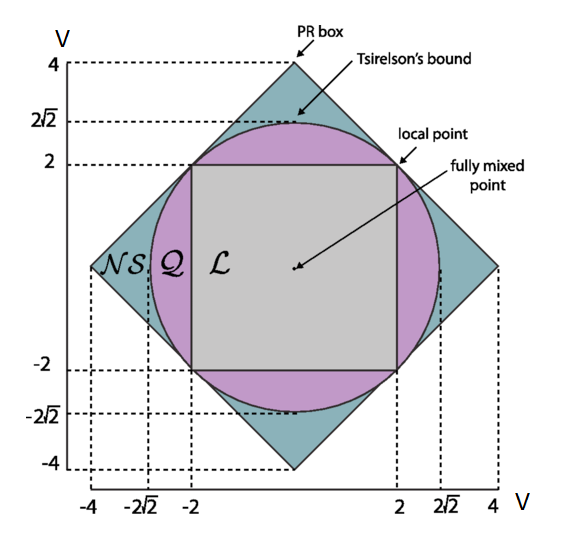
\includegraphics[scale=0.6]{no-signal.png}   
\caption[The no-signalling region of classical physics is bounded above by 2 while the quantum region is bounded above by Tsirelson's bound 2$\sqrt{2}$. The PR box $\cite{PR-1994}$ is the upper bound on the no-signalling region]{The no-signalling region of classical physics is bounded above by 2 while the quantum region is bounded above by Tsirelson's bound 2$\sqrt{2}$. The PR box $\cite{PR-1994}$ is the upper bound on the no-signalling region}
\label{figure:generic}
\end{figure}

Another question comes in mind at this stage is what correlations do exist between the Tsirelson's bound and PR. These are the noisy correlations. As in the GHZ matrix \textbf{p} shown below, there are error parameters associated with the conditional probability distribution $P(a,b|x,y)$. These correlations, as implied before, lie in region that is lower bounded by Quantum and upper bounded by No-signalling. 

At this point, it is important to introduce the concept of Non-local distillation. The objective of $\emph{Non-local Distillation}$ is to amplify the non-locality of a noisy nonlocal resource to form a stronger nonlocal resource using only $local~~operations$.  



\section{Definitions}

A tripartite input-output system characterized by a conditional probability
distribution $P(abc|xyz)$ is \emph{non-signaling} if one cannot communicate 
from one side to the other sides by the choice of the input. This implies that
the marginal probabilities $P(a|x)$, $P(b|y)$, and $P(c|z)$ are independent of the inputs $\left\{ y,z \right\}$, $\left\{ x,z \right\}$, and $\left\{ x,y \right\}$ respectively. 

\begin{align*}
  \sum_{b,c}P(abc|xyz)&=\sum_{b,c}P(abc|xy'z')\equiv P(a|x)\ \forall a,x,y,y',z,z'\\
  \sum_{a,c}P(abc|xyz)&=\sum_{a,c}P(abc|x'yz')\equiv P(a|x)\ \forall a,x,x',y,z,z'\\
  \sum_{b,c}P(abc|xyz)&=\sum_{b,c}P(abc|xy'z')\equiv P(a|x)\ \forall a,x,x',y,y',z\\
\end{align*}


In the no-signalling system as shown above for Alice the probability to receive a on input x is independent of what output the other two parties receive. This is one of the constraints that form the no-signalling polytope. 



We represent a tripartite system by its probability distribution
$P(abc|xyz)$ in matrix notation as
\[\left[
  \begin{array}{ccccc}
    % &ab=00&ab=01&ab=10&ab=11\\\hline
    % xy=000&
     P(000|000)&P(001|000)&P(010|000)&...&P(111|000)\\
    % xy=001&
     P(000|001)&P(001|001)&P(010|001)&...&P(111|001)\\
    % xy=010&
     . &&.&&.\\
     . &&&.&.\\
     . &&&&.\\
     % xy=111&
     P(000|111)&P(001|111)&P(010|111)&...&P(111|111)\\
  \end{array}\right].
\]
The
matrix ${\bf p}$, with its rows having indices $xyz$ and columns  $abc$,
gives the probability with which Alice,Bob, and Charlie output $abc$ on
inputs $xyz$, respectively.  Along with $\emph{positivity}$ and
$\emph{normalization}$  constraints, the no-signalling conditions are enforced on ${\bf p}$ as shown before.
In a general tripartite scenario, the value
attained for a strategy ${\bf p}$ is given by
\begin{eqnarray}
\label{intro:chsheq}
V({\bf p}) = \sum_{f(a,b,c)= g(x,y,z)}P(abc|xyz) - \sum_{f(a,b,c) \neq g(x,y,z)}P(abc|xyz)
\end{eqnarray}
The perfect nonlocal tripartite box is characterized to output a uniform distribution
over the bits $a,b,c$ on inputs $x,y,z$ such that $f(a,b,c)= g(x,y,z)$.

\section{Results}

The bipartite input-output case is unique as it is the only non-local vertex in the bipartite no-signalling polytope. This guarantees that all bipartite non-local correlations can be simulated by that one non-local box, which is Popescu-Rohrlich box $\cite{PR-1994}$, in the following way: 

\begin{eqnarray}
\label{intro:convex}
P_{nl}(ab|xy)= w P_{a \oplus b = xy}(ab|xy)+ (1-w) P_{a \oplus b = xy}(ab|xy).
\end{eqnarray}

where $\emph{w}$ has constraints of normalization and positivity.  

However, the system becomes completely different if we increase the number of parties. 

Pironio $\emph{et al.}$ found 53856 vertices of a tripartite no-signalling polytope that belong to 46 unique classes. For this paper, we are considering a restricted class of tripartite non-local correlations proposed by Greenberger $\emph{et al.}$ $\cite{ghz-1990}$ called $\emph{GHZ}$ correlations. 

We define the $\emph{GHZ}$ non-local box as follows

\[
    p_{abc|xyz=000}= 
\begin{dcases}
    1+\epsilon ,& \text{if } a \oplus b \oplus c = 0\\   
    1-\epsilon, & \text{if } a \oplus b \oplus c = 1\
\end{dcases}
\]


\[
    p_{abc|xyz \neq 000}= 
\begin{dcases}
    1+\delta ,& \text{if } a \oplus b \oplus c = 1\\     
    1-\delta, & \text{if } a \oplus b \oplus c = 0\
\end{dcases}
\]

such that the input \[x \oplus y \oplus z = 0\]

That is to say, the three players Alice, Bob, and Charlie respectively take inputs $x,y,z$ from the set $\left\{000,011,101,110\right\}$ and output $a,b,c$ following the rule \[ a \oplus b \oplus c = x \vee y \vee z \]. The matrix {\bf p} is the following

\begin{displaymath}
%{\bf p}=
\frac{1}{8}
\left( \begin{array}{cccccccc}
1 + \epsilon & 1 - \epsilon & 1 - \epsilon & 1 + \epsilon & 1 - \epsilon & 1 + \epsilon & 1 + \epsilon & 1 - \epsilon  \\ 
1 - \delta & 1 + \delta & 1 + \delta & 1 - \delta & 1 + \delta & 1 - \delta & 1 - \delta & 1 + \delta \\ 
1 - \delta & 1 + \delta & 1 + \delta & 1 - \delta & 1 + \delta & 1 - \delta & 1 - \delta & 1 + \delta \\ 
1 - \delta & 1 + \delta & 1 + \delta & 1 - \delta & 1 + \delta & 1 - \delta & 1 - \delta & 1 + \delta \\ 
\end{array} \right)
\end{displaymath}

The non-local value of ths box is \[V({\bf p}) = 3 \delta + \epsilon\]

We were able to find following \emph{seven} unique distillation protocols and their distillation values. The protocols may be different for the input to the second box. Therefore we only show the inputs to the second box:

\begin{enumerate}
  \item \[V'({\bf p}) = \frac{1}{8}  (-\epsilon^2 + 24\delta^2 + 7\delta\epsilon + \delta + \epsilon) \] for the following protocol
  \[x_2 = x_1 \vee \overline{a_1}~~y_2 = y_1 \vee \overline{b_1}~~z_2 = z_1 \vee \overline{c_1} \] as shown in the FIG. 1 
  \item \[V'({\bf p}) = 3\delta^2 - \epsilon^2 \] for the following protocol
  \[x_2 = \overline{x_1} \wedge \overline{a_1}~~y_2 = y ~~z_2 = z \]
  \item  \[V'({\bf p}) = -\epsilon^2 + \frac{9}{4}\delta^2 - \frac{3}{4}\delta\epsilon \] for the following protocol
  \[x_2 = x_1 \wedge a~~y_2 = y_1 \wedge b~~z_2 = z_1 \wedge c\]
  \item  \[V'({\bf p}) = -\epsilon^2 + \frac{11}{4}\delta^2 - \frac{1}{4}\delta\epsilon \] for the following protocol
  \[ x_2 = x_1 \wedge a~~ y_2 = y_1 \wedge \overline{b}~~z_2 = z_1 \]
  \item  \[V'({\bf p}) =  - \frac{1}{2}\epsilon^2+ \frac{23}{8}\delta^2+ \frac{3}{8}\delta\epsilon+\frac{1}{8}\delta+\frac{1}{8}\epsilon \] for the following protocol
  \[x_2 = x_1 \wedge a~~ y_2 = y_1 \wedge \overline{b}~~z_2 = \overline{a} \vee (x \wedge a) \]
  \item  \[V'({\bf p}) =  -\frac{1}{4}\epsilon^2+\frac{23}{8}\delta^2+\frac{5}{8}\delta\epsilon+\frac{1}{8}\delta+\frac{1}{8}\epsilon \] for the following protocol
  \[x_2 = x_1 \wedge a~~ y_2 = a_1~~ z_2 = \overline{z_1} \wedge c \vee z_1 \]
  \item  \[V'({\bf p}) = -\frac{1}{4}\epsilon^2+3\delta^2+\frac{3}{4}\delta\epsilon\] for the following protocol
  \[ x_2 = x_1 ~~y_2 = y_1 \oplus b_1 ~~z_2 = \overline{z_1} \wedge c \vee z_1 \]
\end{enumerate}

\begin{figure}[t]
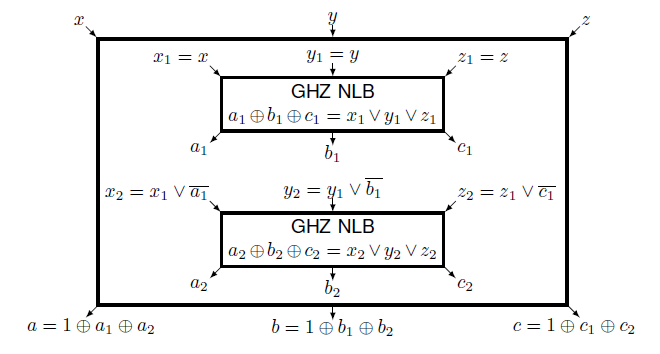
\includegraphics[scale=0.6]{ghz.png}   
\caption[A depth $2$ GHZ distillation protocol.]{A depth $2$ GHZ distillation protocol.}
\label{figure:generic}
\end{figure}

We in particular analyze the protocol 1 and the protocol 2 for their outstanding performances as shown in the  figure 2. 

\begin{figure}[t]
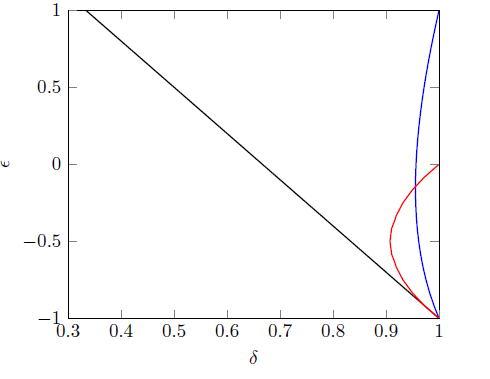
\includegraphics[scale=0.6]{distillation_range.png}   
\caption[It shows the region of distillable GHZ correlations. The black line corresponds to the boundary between local and non-local region. The blue and red contour curves correspond to distilled region using protocol 1 and protocol 2. As shown, it is clear that the protocol 1 covers more range whereas the protocol 2 has a high magnitude]{It shows the region of distillable GHZ correlations. The black line corresponds to the boundary between local and non-local region. The blue and red contour curves correspond to distilled region using protocol 1 and protocol 2. As shown, it is clear that the protocol 1 covers more range whereas the protocol 2 has a high magnitude}
\label{figure:generic2}
\end{figure}



\begin{thebibliography}{17}
  \expandafter\ifx\csname natexlab\endcsname\relax\def\natexlab#1{#1}\fi
  \expandafter\ifx\csname bibnamefont\endcsname\relax
  \def\bibnamefont#1{#1}\fi \expandafter\ifx\csname
  bibfnamefont\endcsname\relax \def\bibfnamefont#1{#1}\fi
  \expandafter\ifx\csname citenamefont\endcsname\relax
  \def\citenamefont#1{#1}\fi \expandafter\ifx\csname url\endcsname\relax
  \def\url#1{\texttt{#1}}\fi \expandafter\ifx\csname
  urlprefix\endcsname\relax\def\urlprefix{URL }\fi
  \providecommand{\bibinfo}[2]{#2}
  \providecommand{\eprint}[2][]{\url{#2}}

\bibitem[{\citenamefont{Bell}(1964)}]{Bell-1964}
  \bibinfo{author}{\bibfnamefont{J.}~\bibnamefont{Bell}},
  \bibinfo{journal}{Physics} \textbf{\bibinfo{volume}{1}},
  \bibinfo{pages}{195} (\bibinfo{year}{1964}).

\bibitem[{\citenamefont{{Popescu} and {Rohrlich}}(1994)}]{PR-1994}
  \bibinfo{author}{\bibfnamefont{S.}~\bibnamefont{{Popescu}}}
  \bibnamefont{and}
  \bibinfo{author}{\bibfnamefont{D.}~\bibnamefont{{Rohrlich}}},
  \bibinfo{journal}{Foundations of Physics}
  \textbf{\bibinfo{volume}{24}}, \bibinfo{pages}{379}
  (\bibinfo{year}{1994}).

  
\bibitem[{\citenamefont{{ghz} et~al.}(2005)\citenamefont{{ghz},
      {Greenberger}, {Horne}, and
      {Shimony}}}]{ghz-1990}
  \bibinfo{author}{\bibfnamefont{D.M.}~\bibnamefont{{Greenberger}}},
  \bibinfo{author}{\bibfnamefont{M.A.}~\bibnamefont{{Horne}}},
  \bibnamefont{and}
  \bibinfo{author}{\bibfnamefont{A.}~\bibnamefont{{Shimony}}},
  \bibinfo{journal}{American Journal of Physics} \textbf{\bibinfo{volume}{71}},
  \bibinfo{pages}{1131-1143} (\bibinfo{year}{1990}),
  \eprint{doi:10.1119/1.16243}.




\end{thebibliography}

\end{document}
